\documentclass[a4paper,12pt]{report}
\usepackage[french]{babel}
\usepackage[T1]{fontenc}
\usepackage[utf8]{inputenc}
\usepackage{lmodern}
\usepackage{microtype}
\usepackage{hyperref}
\usepackage{tabulary}
\usepackage{framed}
\usepackage{fancyhdr}
\usepackage{amsmath}
\usepackage{bbm}


%\usepackage{nopageno}

\newcommand{\latin}[1]{\textit{#1}}

\pagestyle{empty}

\pagestyle{fancy}
\fancyhead{}
\renewcommand{\headrulewidth}{0.5pt}
\fancyhead[R]{\textit{\nouppercase{\rightmark}}}
\fancyfoot{}
\renewcommand{\footrulewidth}{0.5pt}
\fancyfoot[L]{\textit{\nouppercase{\leftmark}}}
\fancyfoot[R]{\thepage}
  
\begin{document}
	\begin{titlepage}
		\vspace*{\stretch{2}}
		\begin{center}
			\large\bfseries\itshape Projet SAR\\
		\end{center}
		\noindent\rule{\linewidth}{3pt}

		\begin{center}
			\Huge\bfseries\itshape RAPPORT\\
		\end{center}
		
		\noindent\rule{\linewidth}{3pt}
		\begin{center}
			\bfseries
			\large Recherche de filtres de Bloom similaires \\
			\large Application à la recherche par mots clés basée sur une DHT
		\end{center}
		\vspace*{\stretch{2}}
		\begin{center}
			Réalisé par \textbf{NDOMBI TSHISUNGU} Christian \& \textbf{DOAN} Cao Sang \\
			Encadre: M. \textbf{MAKPANGOU} Mesaac, Regal
		\end{center}
		\vspace*{\stretch{0.5}}
		\begin{center}
			26 Mars 2015
		\end{center}
	\end{titlepage}

\tableofcontents


\chapter{Introduction}
	{\Huge D}ans ce sujet, on abordera sur les recherches par mots clés. Une fois, on tape un mot ou une chaine de mots, l'application cherche dans la base de données pour trouver la liste des documents qui contient les descriptions correspondantes avec ces mots clés.
	
	Dans la base de données qui contient des grosses masses de donées, les index sont basés sur les descriptions des documents. Chaque mot est une clé, chaque clé contient une liste des documents ayant ce mot. Au contraire à la liste normale, le mot clé est le nom du document et il contient la liste des mots qui se trouvent dans la description de ce document. Par exemple, le mot {\em PSAR : le projet pour les étudiants du M1}, normalement, le mot clé est {\em PSAR}, donc il contient sa description {\em le projet pour les étudiants du M1}, mais dans cette liste, les mots clés sont {\em le, projet, pour, les, étudiants, du, M1} et chaque mot contient le mot {\em PSAR}. On s'appelle la {\em liste inversée}.
	
	Du coup, on utilise les tables de hachage distribuées (DHT) pour stocker les listes inversées. L'avantage d'utilisation de ces tables est que la complexité est égale à $ \theta ${\em (1)} car on trouve directement l'élément que l'on recherche. La statégie de distribution des listes inversées la plus utilisée (appelée partionnement vertical) consiste à associer à chaque terme une clé qui désigne le pair qu stocke la liste inversée associée à ce terme. Une fois que l'on lance la recherche sur les documents qui sont satisfaits à l'ensemble des mots que l'on a saisi, le système doit chercher pour chaque mot dans cet ensemble la liste des documents qui le contiennent, et puis fait l'intersection des listes inversées retrouvées. 

\chapter{Projet}
\section{Marché}
		Il existe actuellement plusieurs moteurs de recherche par mots clés sur le marché. Il est toujours nécessaire d’améliorer les recherches en minimisant le temps de réponse et le coût de recherche, d’autant plus que les besoins de recherche deviennent très importants lorsqu’on exploite des bases de données de plus en plus grande et complexe. L’application que nous développerons doit répondre explicitement à ces exigences.
		
	\section{Contexte et objectifs}
		Comme l’application FreeCore\cite{freecore}, qui utilise le filtre de Bloom pour faciliter la recherche par mot clé, le but de notre projet est d'explorer d’autres solutions basées sur une recherche de filtre de Bloom similaires.  Chaque filtre  de  Bloom  sera vu  comme  un  point  dans  un  espace à n dimensions  plutôt  qu'une  concaténation de  n mots binaires. On détermine ensuite une relation de proximité et on exploite les algorithmes de recherche des filtres similaires pour réduire l'ensemble de filtres à examiner.
		
	\section{Enoncé du besoin}
		Comme FreeCore, l’application exploitera les propriétés des filtres de Bloom. Il  permettra d’une part, de stocker les publications dans un fichier $VA\_file$ (put). Et d’autre part, d’effectuer des recherches de contenus par mots clés (search).
	\subsection{Stockage et indexation des publications}
	L’application permet de rechercher des publications qui contiennent tous les mots clés de la requête de façon optimale en utilisant le filtre de Bloom. Elle doit :
	\begin{itemize}
	
	\item créer un filtre de Bloom correspondant à la description de la publication, 
	\item créer un vecteur de n dimensions.
	\item créer les lieux où on stocke les différents documents,
	\item à partir d'un fichier de test, classer et indexer les documents dans les lieux correspondants,		
	\item ajouter un nouveau document à partir d'un filtre de Bloom,				\end{itemize}
	
	\subsection{Recherche de contenus}
	Pour la recherche l’application créera un Filtre de Bloom des mots clés, représentants notre critère de recherche, c’est-à-dire les mots clés et devra :
	\begin{itemize}
		\item recherche un document à partir du filtre de Bloom,
 		\item utilise le vecteur approximatif pour indexer et rechercher.
	\end{itemize}
	
En outre, l’application doit assurer les services suivants :

	\begin{itemize}
	\item afficher les messages d'erreurs, s'il en existe,	
	\item afficher les états de l'application,	
	\item interagir avec l'utilisateur,
	\item faciliter les tests en utilisant les fichiers de test ou en utilisant les entrées saisit par l'utilisateur.
	\end{itemize}
	\begin{description}
		\item[Note :] Nous ne traiterons pas les erreurs  possibles obtenues en cas de faute de frappe ou de faute d’orthographe, ni la différence de genre et de nombre des mots clés. Qui pourront faire objet d’une suite de ce travail.
			\end{description}

\chapter{Filtre de Bloom}
	{\huge \itshape U}n filtre de Bloom est une structure de données probabiliste compacte inventée par Burton Howard Bloom en 1970\footnote{Wikipédia}. L'avantage d'utilisation de filtre de Bloom est que cette technique nous permet de savoir avec certitude que l'élément n'est pas présenté dans l'ensemble d'élément, c'est-à-dire il ne faut pas y avoir de faux négatif mais il peut y avoir des faux positifs. On ne peut savoir qu'avec une certaine probabilité, l'élément peut être présent dans l'ensemble. Ce qui réduit d'une manière considérable les entrées lorsqu'on fait une recherche dans une masse de données. En plus, la taille de filtre est fixe et indépendante du nombre d'éléments contenus, par contre, plus déléments plus de faux positifs.
	
	En réalité, le filtre de Bloom a un structure très simple, un tableau B de \textit{m} bits associé à $i$ fonctions de hachage $h_i$, $0 \leq i \leq m - 1$ permettant de mapper tout élément de l'ensemble à une des $m$ cases du tableau. Ces fonctions de hachage ont une répartition uniforme des éléments de l'ensemble sur le tableau, et évidemment, doivent avoir une répartition différente. Au départ, le filtre représente un ensemble vide, et toutes les cases sont à 0.
	
	Pour chaque clé $k$ à ajouter à B, au lieu de se contenter de mettre à vrai la case B. $h(k)$ avec une seule fonction de hachage comme on le fait classiquement, on va mettre à vrai les $m$ cases B. $h_i(k)$. Le principe étant que la probabilité que deux clés différentes aient les mêmes $m$ valeurs pour leurs fonctions de hachage est faible.
	
	Pour savoir si une clé est présente, on s'assura que les $m$ cases de la table B correspondant aux valeurs des $m$ fonctions de hachage sont posisitionnées à $1$. Ce filtre est utile pour déterminer si un élément ne fait pas partie d'un ensemble, afin par exemple pour définir rapidement d'un traitement lourd lors de vérifier qu'une personne ne fasse pas partie d'une liste noire: d'abord, une vérification rapide avec le filtre de Bloom, puis en cas de potentiel posistif, un vérification plus certaine avec la comparaison dans la base de données.
	
	Le filtre de Bloom a quelques désavantages comme par exemple pour supprimer un élément dans l'ensemble de données, il nous faut reconstruire le filtre, en plus les faux posisitifs augmentent avec le nombre d'éléments présents dans l'ensemble. Nombreuses solutions utilisent des techniques probabilistes pour réduire le traitement d'information et leur coût.
	
	Le filtre de Bloom et leurs variantes sont largement utilisés dans divers systèmes distribués. Plusiseurs recherches récentes et beaucoup de nouveaux algorithmes ont été proposés pour les systèmes distribués qui sont directement ou indirectement basés sur Bloom filtres\cite{theory-and-practice-of-bloom-filters-for-distributed-systems}.
	
\newtheorem{algorithme}{Algorithme}
\begin{algorithme}
	Insertion dans le filtre de Bloom
\end{algorithme}

\begin{flushleft}
	\begin{framed}
		\textbf{IN:} \textit{x} objet à insérer dans le filtre de Bloom \textit{B}\\
		\textbf{FUNCTION:} \textit{insert(x)}\\
		\textbf{OUT:} $\emptyset$
		\noindent\rule{\linewidth}{0.5pt}

		\begin{tabbing}
			\textbf{for} \= $i = 0 ... k - 1$ \textbf{do}\\
					\> $j \leftarrow h_i(x)$\\
					\> \textbf{if} \= $B_j == 0$ \textbf{then}\\
					\> \> $B_j \leftarrow 1$\\
					\> \textbf{end}\\
			\textbf{end}
	    	\end{tabbing}		
	\end{framed}
\end{flushleft}
	
	Par exemple, supposons que nous souhaitions ajouter la clé "computer" dans la table B de taille 16 bits, que nous ayons 4 fonctions de hachage $ h_i, 0 \leq i < 4 $ et que $ h_0("computer") = 3$, $ h_1("computer") = 8$, $ h_2("computer") = 15$, $h_3("computer") = 10$, $h_4("computer") = 11 $. Donc, l'état de la table $ B $ après l'insertion sera:
	\begin{table}[!h]
		\centering		
		\begin{tabular}{|l|*{14}{c|}r|}
		\multicolumn{1}{c}{{\scriptsize 15}} &\multicolumn{1}{c}{}&\multicolumn{1}{c}{}&\multicolumn{1}{c}{}&\multicolumn{1}{c}{}&\multicolumn{1}{c}{}&\multicolumn{1}{c}{}&\multicolumn{1}{c}{}&\multicolumn{1}{c}{}&\multicolumn{1}{c}{}&\multicolumn{1}{c}{}&\multicolumn{1}{c}{}&\multicolumn{1}{c}{}&\multicolumn{1}{c}{}&\multicolumn{1}{c}{}&\multicolumn{1}{c}{{\scriptsize 0}}\\
		\hline
			1 & 0 & 0 & 0 & 1 & 1 & 0 & 1 & 0 & 0 & 0 & 0 & 1 & 0 & 0 & 0 \\
		\hline
		\end{tabular}
		\caption{Exemple filtre de Bloom}
		\label{filtredeBloom/exemple}
	\end{table}
	
\begin{algorithme}
	Test d'appartenance d'un élément dans le filtre
\end{algorithme}

\begin{flushleft}
	\begin{framed}
		\textbf{IN:} \emph{x} objet à tester dans le filtre de Bloom \textit{B}\\
		\textbf{FUNCTION:} \textit{ismember(x)}\\
		\textbf{OUT:} $bool$

		\noindent\rule{\linewidth}{0.5pt}

		\begin{tabbing}
			$m \leftarrow true$\\
			$i \leftarrow 0$\\
			\textbf{while} \= $m$ \&\& $i \leq k - 1$ \textbf{do}\\
					\> $j \leftarrow h_i(x)$\\
					\> \textbf{if} \= $B_j == 0$ \textbf{then}\\
					\> \> $m \leftarrow false$\\
					\> \textbf{end}\\
					\> $i \leftarrow i + 1$\\
			\textbf{end}
			\textbf{return} $m$\\
	    	\end{tabbing}		
	\end{framed}
\end{flushleft}

\begin{figure}[!htbp]
	\centering
	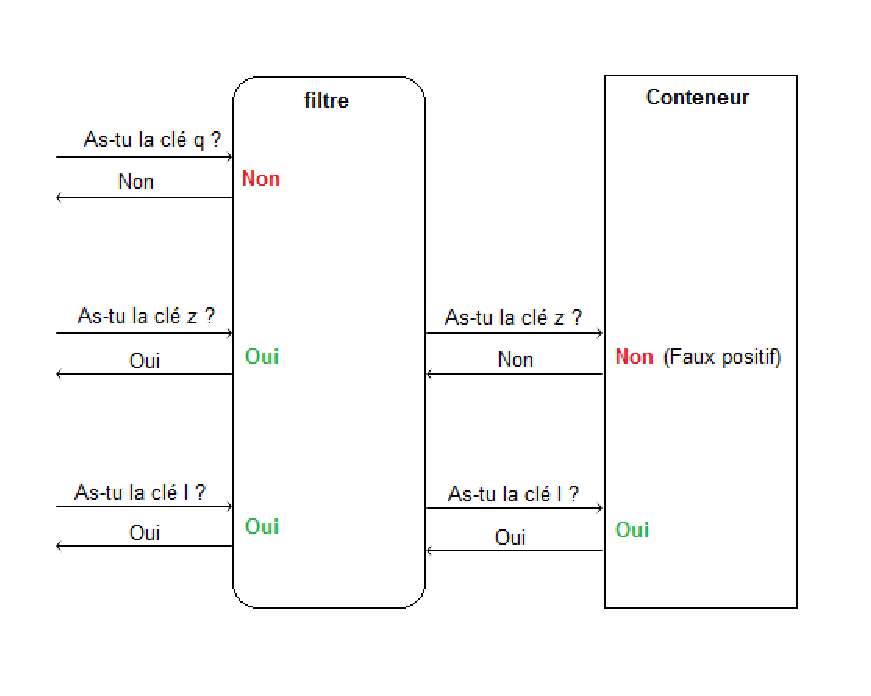
\includegraphics[width=12cm]{ismember.eps}
	\caption{isMember?}
\end{figure}	

	
	
	
	
	
	
	
	
	
	
	
	
	
	
	
	
	
	
	
	
	
\begin{thebibliography}{2}
	\bibitem{freecore}
		Mesaac Makpangou, Bassirou Ngom, Samba Ndiaye : 
		\textbf{\textit{Freecore: Un substrat d'indexation des filtres de Bloom fragmentés pour la recherche par mots clés}}.
		ComPAS'2014, Apr 2014, Neuchâtel, Switzerland
	\bibitem{theory-and-practice-of-bloom-filters-for-distributed-systems}
   		Sasu Tarkoma, Christian Esteve Rothenberg, and Eemil Lagerspetz :
  		 \textbf{\textit{Theory and Practice of Bloom Filters for Distributed Systems}}.
		Communications Surveys \& Tutorials, IEEE. pp. 131 – 155. Fevrier. 2012
\end{thebibliography}


\end{document}